\documentclass[10pt]{article}

\usepackage[accepted]{rlc}
% If accepted, instead use the following line for the camera-ready submission:
%\usepackage[accepted]{rlc}
% To de-anonymize and remove mentions to RLC (for example, for posting to preprint servers), instead use the following:
% \usepackage[preprint]{rlc}

\usepackage{array}
\usepackage{amsmath}
\usepackage{amsthm}
\usepackage{amsbsy}
\usepackage{amssymb}
\newtheorem{definition}{Definition}
\usepackage{graphicx}
\usepackage{mathtools}
\usepackage{nicefrac}
\usepackage{bm}
\usepackage{enumitem}
\usepackage{mpemath}
\usepackage{tcolorbox}
\usepackage[capitalize,noabbrev]{cleveref}
\usepackage{theoremref}
\usepackage{thmtools}
\usepackage{thm-restate}
\usepackage{algorithm}
\usepackage{algpseudocode}
\usepackage{tikz}
\usepackage{subcaption}
\usepackage{hyperref}
\usepackage{dsfont}
\usepackage{bbm}


\bibliographystyle{abbrvnat}
\usepackage[framemethod=default]{mdframed}

\renewcommand{\cite}{\citep}

\renewcommand{\algorithmicrequire}{\textbf{Input:}}
\renewcommand{\algorithmicensure}{\textbf{Output:}}
\newcommand{\cvar}{\text{CVaR}}
\newcommand{\cvaralpha}{\text{CVaR}_\alpha}
\newcommand{\var}{\text{VaR}}
\newcommand{\varalpha}{\text{VaR}_\alpha}


\theoremstyle{plain}
\newtheorem{theorem}{Theorem}
\newtheorem{lemma}{Lemma} 
\newtheorem{proposition}{Proposition}
\newtheorem{assumption}{Assumption}
\theoremstyle{remark}
\newtheorem{example}{Example}

% \newcommand{\mm}[1]{\textcolor{magenta}{[#1]}}
% \newcommand{\db}[1]{\textcolor{blue}{[DB: #1]}}
% \newcommand{\gersi}[1]{\textcolor{red}{[#1]}}
% \newcommand{\s}[1]{\mathcal{#1}}

\DeclareMathOperator{\ext}{ext}
\DeclareMathOperator*{\essinf}{ess\,inf}

% \setlength{\parskip}{3mm plus 1mm minus 1mm}
% \setlength{\parindent}{0pt}

\title{Survey on Risk-Averse Reinforcement Learning}
\author{Gersi Doko \\
        Gersi.Doko@unh.edu \\}


\begin{document}

\maketitle

\section{Introduction}

Reinforcement learning (RL) is a powerful framework for developing agents that can learn to make decisions in complex, uncertain environments~\cite{sutton2018, Puterman1994, MEHTA2007237, Hall2018}.
The core goal of RL is to tractably compute an optimal policy for acting in such an environment. A key challenge in RL is 
that the environment is often stochastic, and decisions made now can affect state distributions encountered in the
future. Choosing an objective function that accurately captures the desired behavior of the agent is a difficult task.

We would hope the objective that an RL agent aims to optimize would consider the `risk' of the actions it takes. Before even phrasing such an objective, one first needs to consider how to quantify risk into a numerical value. A value that encapsulates the uncertainty of the outcome of an action,
so that an agent can distinguish between actions that are risky and those that are safe.

There is a vast field of research that focuses on developing risk measures~\cite{follmer2016, Hau2023OnDP, Bauerle2011, howard1972}. The goal of a risk measure is to quantify the uncertainty of a random variable, often while being interpretable and computationally tractable. The intersections of risk and reinforcement learning is the topic of this review, where we will explore the field of risk-averse reinforcement learning.

One must be cautious when optimizing a risk sensitive objective due to the
common pitfalls that arise even in the published
literature~\cite{Hau2023OnDP}. Many risk measures do not satisfy the
properties common to expectation. And therefore many blunders found in the literature can be attributed to either
misunderstanding of the optimization literature or the risk measure itself.

\section{Preliminaries}

In order to introduce the concepts of risk-averse reinforcement learning, we first need to define some basic concepts in probability theory and reinforcement learning.

Unless explicitly stated we assume all variables are discrete, and finite. We adopt the notation that all random
variables are adorned with a $\tilde{\cdot}$ unless obvious from context, all matrices are capitalized, and all sets are calligraphic.

We adopt the common notation that $\Delta^n$ denotes the $n$-dimensional simplex. For two sets $A$ and $B$, $A^B$ denotes the set of all functions from $B$ to $A$. For a set $A$, $|A|$ denotes the cardinality of $A$.

The environment is a Markov Decision Process (MDP) defined by a tuple $\mathcal{M} = (\mathcal{S}, \mathcal{A}, \mathcal{P}, r, \gamma)$ where
\begin{itemize}
        \item $\mathcal{S}$ is the state space,
        \item $\mathcal{A}$ is the action space,
        \item $\mathcal{P} : \mathcal{S} \times \mathcal{A} \to \Delta^\mathcal{S}$ is the transition probability function,
        \item $r : \mathcal{S} \times \mathcal{A} \to \Real$ is the reward function,
        \item $\gamma \in [0, 1$ is the discount factor.
\end{itemize} 
Finally, we define the set of all deterministic policies $\Pi_D = \mathcal{A}^\mathcal{S}$. 
And the set of all randomized policies $\Pi_R = {[\Delta^\mathcal{A}]}^\mathcal{S}$.
We encourage the reader to refer to~\cite{Puterman1994} for a more detailed introduction to MDPs.

\section{Risk and Reward}\label{sec:risk-and-reward}

\begin{definition}[Risk Measure]\label{def:risk}
        A Risk Measure is a mapping from a random variable $\tilde{x}$ to a real number. Quantifying the uncertainty of an outcome.
        Given a metric space ($\Omega$, $\mathcal{F}$, $P$), a risk measure is a function $\psi: \mathcal{X} \to \Real$. Satisfying
        \begin{enumerate}
          \item Monotonic: $\tilde{x} \leq \tilde{y} \implies \psi(\tilde{x}) \leq \psi(\tilde{y})$
          \item Translation Invariance: $\psi(\tilde{x} + c) = \psi(\tilde{x}) + c \quad \forall c \in \Real$
        \end{enumerate}
\end{definition}

\begin{definition}[Coherent Risk Measure]\label{def:coherent-risk-measure}
        Given a metric space ($\Omega$, $\mathcal{F}$, $P$), a coherent risk measure is a function $\psi: \mathcal{X} \to \Real$. Satisfying
        \begin{enumerate}
                \item All items in definition~\ref{def:risk}
                \item Sub-additivity: $\psi(\tilde{x} + \tilde{y}) \leq \psi(\tilde{x}) + \psi(\tilde{y})$
                \item Positive Homogeneity: $\psi(\lambda \tilde{x}) = \lambda \psi(\tilde{x})$ for $\lambda \in \Real_+$
        \end{enumerate}
\end{definition}

\begin{proposition}\label{prop:coherent-convex}
        All coherent risk measures are convex risk measures.
        \begin{proof}
          Let $\psi$ be a coherent risk measure. Then for $\tilde{x}, \tilde{y} \in \mathcal{X}$ and $\lambda \in [0, 1]$ we have
                \begin{align*}
                        \psi(\lambda \tilde{x} + (1 - \lambda) \tilde{y}) &\leq \psi(\lambda \tilde{x}) + \psi((1 - \lambda) \tilde{y}) &&\text{Sub-Additivity}\\
                        &= \lambda \psi(\tilde{x}) + (1 - \lambda) \psi(\tilde{y}) &&\text{Positive Homogeneity}\\
                \end{align*}
        \end{proof}
\end{proposition}

It is important to note the converse of Proposition~\ref{prop:coherent-convex} is not true. That is, not all convex risk measures are coherent. This is due to positive homogeneity.

\begin{definition}[Variance]\label{def:variance}
        The variance of a random variable $X$ is defined as 
        \[
                \text{Var}(\tilde{x}) = \mathbb{E}[{(\tilde{x} - \mathbb{E}[\tilde{x}])}^2].
        \]
\end{definition}

\begin{definition}[Expectation]\label{def:expectation}
        A common risk measure is the expectation of a random variable. Given a random variable $X: \Omega \to \Real$, the expectation of $X$ is defined as
        \[
          \mathbb{E}[\tilde{x}] = \sum_{\omega \in \Omega} \tilde{x}(\omega) \mathbb{P}(\omega).
        \]
\end{definition}

\begin{definition}[Value-at-Risk --- $\varalpha$]\label{def:var}
        For $\alpha \in [0, 1]$, the Value-at-Risk of a random variable 
        $\tilde{x}$ at risk-level $\alpha$ is defined as
        \[
                \normalfont{\varalpha(\tilde{x})} = \sup_{t \in \Real} \left\{ \mathbb{P}(\tilde{x} < t) \leq \alpha \right\} = \inf_{t \in \Real} \left\{ \mathbb{P}(\tilde{x} \leq t) > \alpha \right\}.
        \]
\end{definition}

\begin{definition}[Conditional Value-at-Risk --- $\cvaralpha$]\label{def:cvar}
        For $\alpha \in [0, 1]$, the Conditional-Value-at-Risk of a random variable 
        $\tilde{x}$ with pdf $p$ at risk-level $\alpha$ is defined as
        \[
                \normalfont{\cvaralpha(\tilde{x})} = \sup_{t \in \Real} \left\{ t - \frac{1}{\alpha} \mathbb{E}{[t - \tilde{x}]}_+ \right\} =
                \inf_{\xi \in \Delta^n} \left\{ \xi\tr x \mid \alpha \cdot \xi \leq p \right\}.
        \]
\end{definition}

From the definitions of both $\var$ and $\cvar$ we can see that $\var_1[\tilde{x}] = \infty$ and $\cvar_1[\tilde{x}] = \mathbb{E}[\tilde{x}]$.
$\cvar_0[\tilde{x}] = \essinf[\tilde{x}]$ where $\essinf[\tilde{x}]$ is the essential infimum of $\tilde{x}$ with pdf $p$ (smallest value with nonzero probability).


\begin{figure}[ht!]
        \begin{subfigure}[t]{0.5\textwidth}
                \centering
                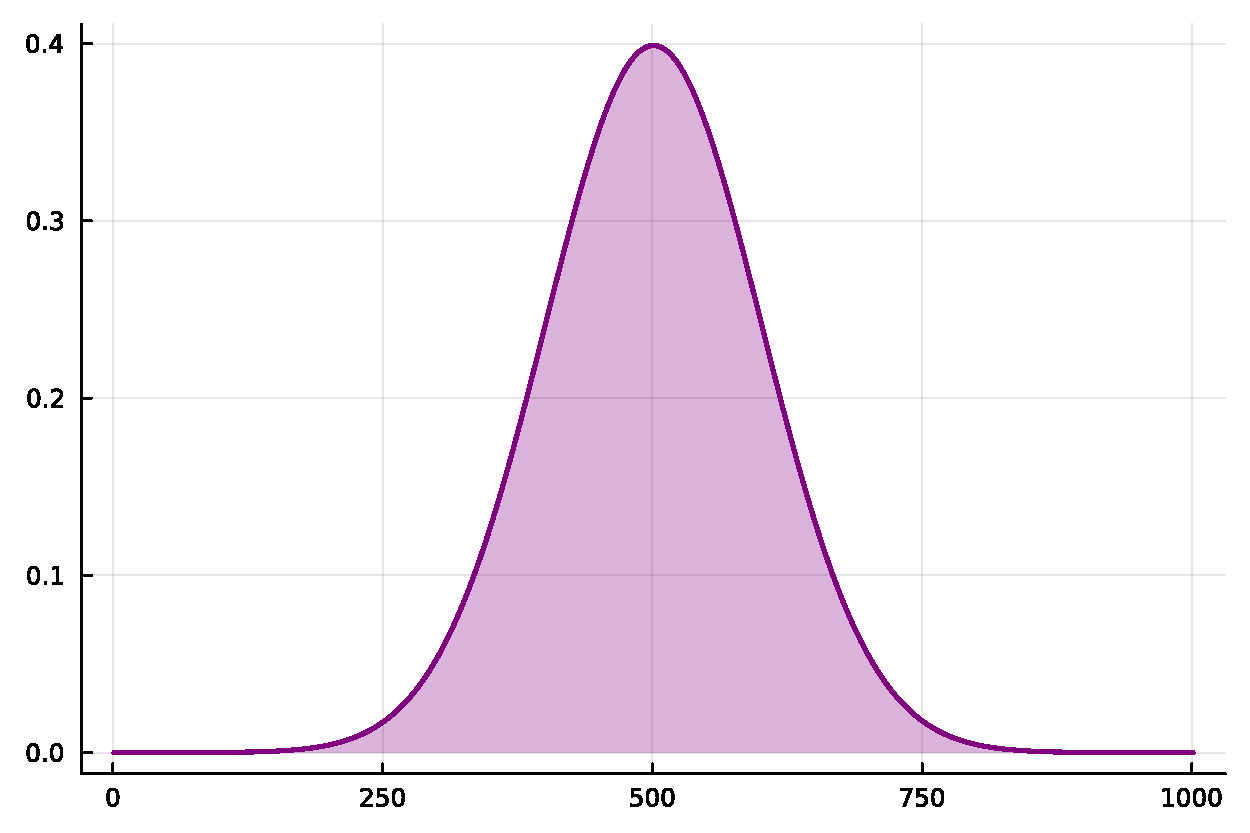
\includegraphics[width=0.7\linewidth]{julia_figures/normal.pdf}
                \caption{$\mathcal{N}(0,1)$}\label{fig:normal}
        \end{subfigure}
        \begin{subfigure}[t]{0.5\textwidth}
                \centering
                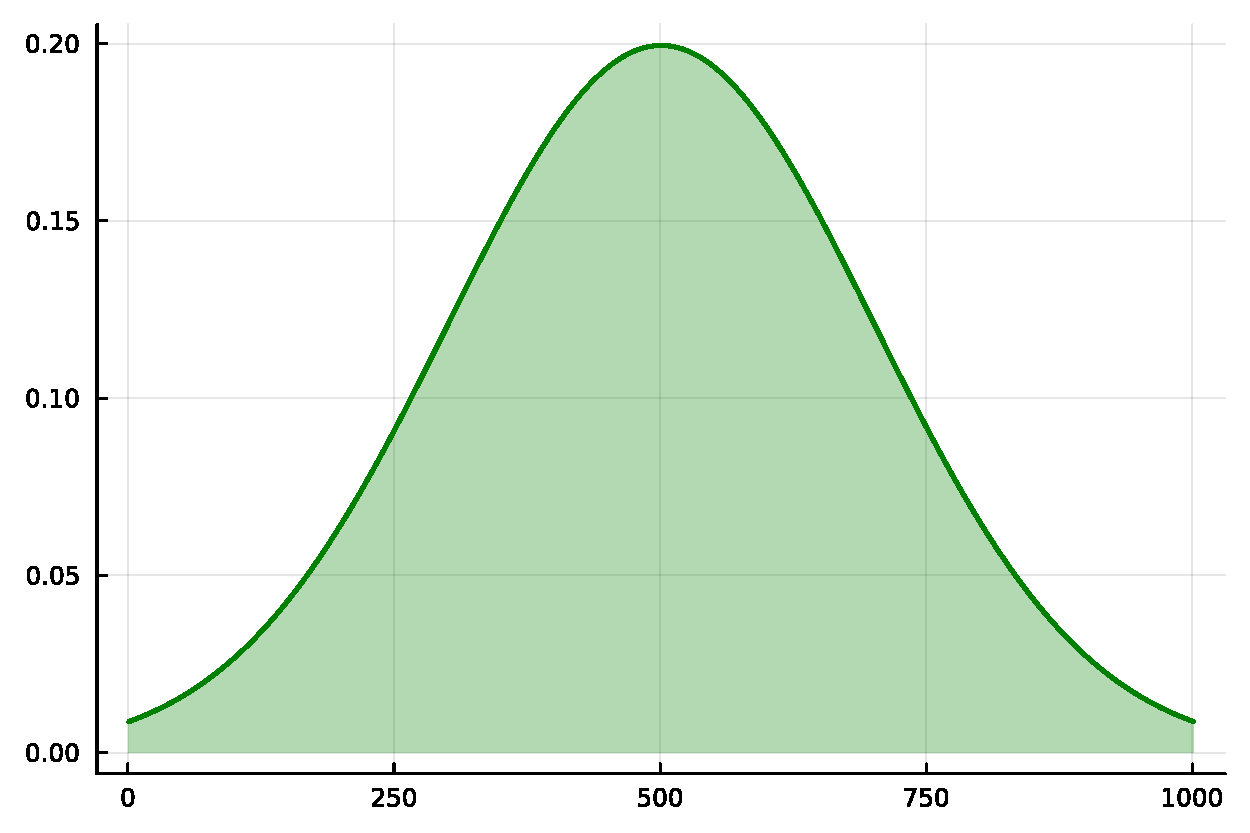
\includegraphics[width=0.7\linewidth]{julia_figures/normal_wide.pdf}
                \caption{$\mathcal{N}(0,2)$}\label{fig:normal_wide}
        \end{subfigure}
        \begin{subfigure}[t]{1.0\textwidth}
                \centering
                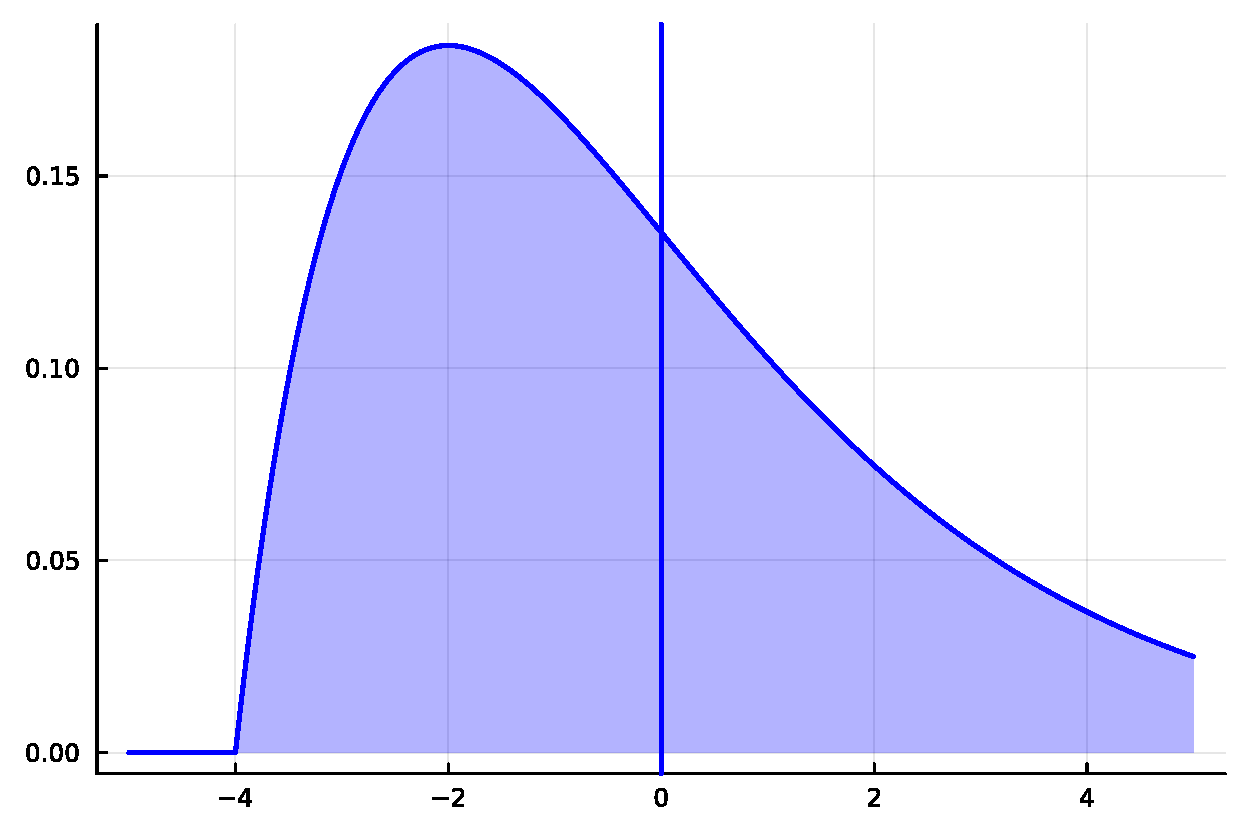
\includegraphics[width=0.4\linewidth]{julia_figures/gamma.pdf}
                \caption{$\Gamma(2,2) - 4$}\label{fig:gamma}
        \end{subfigure}
        \caption{Probability density functions (PDFs) of various distributions. All with a shared mean of 0 denoted by the vertical line.}\label{fig:pdfs}
\end{figure}

The simplest, and most accessible coherent risk measure is the expectation operator $\mathbb{E}$, see definition~\ref{def:expectation}.\label{sec:explanation-of-why-risk-measures-are-important}
Expectation often ignores tail risk, and reduces a random variable to its mean as seen in Figure~\ref{fig:pdfs}.
Expectation also cannot easily be parameterized to capture the risk preferences of the agent.
As such


Our introduction of the concept of risk is largely inspired by the influential work of~\cite{follmer2016}. We refer the reader there for a more delicate and detailed treatment of risk measures and their subsequent properties.

\section{Vanilla Reinforcement Learning}\label{sec:vanilla-reinforcement-learning}

In order to make decisions one must adopt a policy which prescribes the agent's behavior.
A policy is a mapping from states to actions, and the goal of reinforcement learning is to find an optimal policy that maximizes the expected return.
Policies may depend on time, and the agent may have a horizon of $T$ time steps to act. 
In this paper we assume a finite horizon, with each $s \in S$ having a time component, thus we omit the subscript $t$ on all variables for simplicity.

\begin{definition}[Finite Horizon Expected Discounted Return]
        Given a policy $\pi : \mathcal{S} \to \mathcal{A}$ the expected finite horizon discounted return $\rho(\pi)$ can be defined as
        \[ 
          \rho(\pi) = \mathbb{E}_{\pi, \mathcal{P}} \left[ \sum_{t=0}^{T} \gamma^t r(\tilde{s}_t, \pi(\tilde{s}_t)) \right].
        \]
        Where $\tilde{s}_0 \sim p_0$ and $\tilde{s}_{t+1} \sim \mathcal{P}(s_t, \pi(s_t))$, $\gamma$ is the discount factor, and $T$ is the time horizon.
\end{definition}

\begin{definition}[Objective of Reinforcement Learning]\label{def:rl_obj}
        The objective of reinforcement learning (RL) is as follows
        \[
        \max_{\pi \in \Pi} \rho(\pi). 
        \]
\end{definition}

\begin{definition}[Optimal Policy]\label{def:optimal_policy}
        An optimal policy $\pi^\star \in \argmax_{\pi \in \Pi} \rho(\pi)$.
\end{definition}

\begin{definition}[Optimal Value Function]\label{def:optimal_value_function}
        Given an optimal policy $\pi^\star$, the optimal value function starting at time $l \in [0\ldots T-1]$ $V^\star_l = V^{\pi^\star}_l : \mathcal{S} \to \Real]$ is defined as
        \[
          V^\star_l(s) = r(s,\pi(s)) + \mathbb{E}_{\mathcal{P}} \left[ \sum_{t=l+1}^{T} \gamma^t r(\tilde{s}_t, \pi^\star(\tilde{s}_t)) \right].
        \]
        Where $\tilde{s}_{l+1} \sim \mathcal{P}(s, \pi(s))$ and
        \[
          V^\star_T(s) = r(s).
        \]
\end{definition}

Notice in~\ref{def:optimal_policy} that the optimal policy may not be unique, as there may be multiple policies that achieve the same expected return. Notice also that our definition of the value function presupposes the existence of an optimal policy and requires that policy in order to derive the value function. For a general MDP this need not be the case, and we refer the reader to~\cite{Puterman1994} for a description on the deep and rich relationship between value functions and policies which we do not embark on here.


\subsection{Dynamic Programming}
A common approach to solving the objective of reinforcement learning is to use dynamic programming. Dynamic programming is a method for solving complex problems by breaking them down into simpler sub-problems. In the context of reinforcement learning, dynamic programming is used to compute the optimal value function and policy.

\begin{definition}[Bellman Equation]\label{def:bellman}
        Given a policy $\pi : \mathcal{S} \to \mathcal{A}$, the Bellman equation for the value function is defined as
        \[
                V^\pi_l(s) = r(s, \pi(s)) + \gamma \mathbb{E}_{s' \sim \mathcal{P}(s, \pi(s))} [V^\pi_{l+1}(s')].
        \]
\end{definition}
The Bellman equation is a recursive equation that decomposes the value function into two parts: the immediate reward and the value of the next state. While we
consider deterministic policies in our definition here, the Bellman equation can be extended to randomized policies as well through the use of an expectation operator.

\begin{definition}[Bellman Optimality Equation]\label{def:bellman_optimality}
        Given a policy $\pi : \mathcal{S} \to \mathcal{A}$, the Bellman optimality equation for the value function is defined as
        \[
                V^\star_l(s) = \max_{a \in \mathcal{A}} \left\{ r(s, a) + \gamma \mathbb{E}_{s' \sim \mathcal{P}(s, a)} [V^\star_{l+1}(s')] \right\}.
        \]
\end{definition}

\begin{proposition}\label{prop:optimal_policy_value}
        There exists an optimal policy $\pi^\star$ such that $V^\star_l(s) = V^{\pi^\star}_l(s)$ for all $s \in \mathcal{S}$ and for all $l \in [1\ldots T]$.
\end{proposition}

While Proposition~\ref{prop:optimal_policy_value} seems obvious, and indeed the proof is trivial by contradiction. We include it here to illustrate a key idea which allows our goal of finding an optimal policy that maximizes the expected return by dynamic programming.

We urge the reader to consider the work of~\cite{sutton2018} for a more detailed introduction to reinforcement learning beyond dynamic programming.
For a more detailed account of the theoretical results glossed over in this summary, please see~\cite{Puterman1994}.

\section{Risk-Averse Reinforcement Learning}

Consider the return function $\rho(\pi)$, which is of key importance in reinforcement learning~\ref{def:rl_obj}. 
The inner expectation of $\rho(\pi)$ is a risk measure, as such one can imagine replacing the expectation
with a different risk measure $\psi$.

However, expectation is already a coherent risk measure, so the question arises, why would one want to replace it with a different risk measure? 
We refer the reader to the discussion in Section~\ref{sec:explanation-of-why-risk-measures-are-important} of this
work and to the work of~\cite{Bauerle2011, follmer2016, howard1972} for further motivation. 

In contrast to Section~\ref{sec:vanilla-reinforcement-learning} we now consider the set of all policies to be history dependent randomized policies instead of stationary deterministic policies. That is to say, from now on 
\[ 
        \Pi = \Pi_{\text{HR}} = \left\{ \pi : {[\mathcal{S} \times \mathcal{A}]}_{0}^{t} \to \Delta^\mathcal{A} \right\}.
\]
This group of policies is more general than the set of deterministic policies, and allows for a more flexible representation of the agent's behavior.
For the particular reader who is interested in why we only considered stationary deterministic policies in Section~\ref{sec:vanilla-reinforcement-learning} we refer them to the work of~\cite{Puterman1994} (Proposition 4.4.3).

There has been prior work on embedding a utility function within the expectation, perhaps one encoding the preferences of an agent who
desires higher returns less and less~\cite{howard1972}.\todo{Ask Marek why this doesn't suffice} 

\begin{definition}[Risk-Averse Reinforcement Learning]\label{def:risk_averse_rl}
        Given a risk measure $\psi$, the objective of risk-averse reinforcement learning is as follows
        \[
                \max_{\pi \in \Pi} \hat{\rho}(\pi) = \max_{\pi \in \Pi} \psi_\mathcal{P} \left( \sum_{t=1}^{T} \gamma^t r(\tilde{s}_t, \pi(\tilde{h}_t)) \right).
        \]
        Where $\tilde{s}_1 \sim p_0$ and $\tilde{s}_{t+1} \sim \mathcal{P}(s_t, \pi(\tilde{h}_t))$, $\tilde{h}_t = (\tilde{s}_1, \tilde{a}_1, \ldots, \tilde{s}_{t-1}, \tilde{a}_{t-1})$ and $\pi(\tilde{h}_t) \in \Delta^\mathcal{A}$.
\end{definition}

\begin{definition}[Optimal Risk-Averse Policy]\label{def:optimal_risk_averse_policy}
        An optimal risk-averse policy $\pi^\star \in \argmax_{\pi \in \Pi} \hat{\rho}(\pi)$.
\end{definition}

Here however we depart from the standard procedure of defining the value function recursively as would be required for dynamic programming and as was done in Section~\ref{sec:vanilla-reinforcement-learning}.
The reason for this is that the risk measure $\psi$ does not usually satisfy the tower property, which is a key property for the Bellman equation to hold.

An open research question is how to decompose different risk measures as in Section~\ref{sec:risk-and-reward} into a recursive form that would allow for dynamic programming to be used for policy optimization.
This topic is a difficult one, and we refer the reader to the work of~\cite{Hau2023OnDP, Bauerle2011, follmer2016} for a more detailed treatment of this topic.


\section{Methods}

\bibliography{main.bib}

\end{document}
